% --------------------------------------------------------------------------
% Шаблон презентации в стилистике Университета ИТМО
% Версия шаблона 2.1. Также шаблон доступен на сайтах:
% https://www.overleaf.com/read/rpkkfchcnbsc
% https://www.overleaf.com/latex/templates/itmo-beamer-theme/fpttrgnmqwsb
% https://github.com/AlexZabashta/ITMO-Beamer-theme
% --------------------------------------------------------------------------

% Внимание!!!
% Этот документ создан для примера использования beamer стиливика.
% Не стоит воспринимать его как урок Latex или beamer!
% Ознакомьтесь с возможностями Latex и beamer (хотя бы базовыми) отдельно.

\documentclass[aspectratio=169]{beamer}
\usepackage{presentation_style}
\usepackage{appendixnumberbeamer}

% Без этой команды он иногда ругается.
\hypersetup{unicode=true}

% Пакет для "русификации" Latex.
\usepackage[english,russian]{babel}

% Чтобы адекватно работало копирование текста из полученной .pdf-ки.
\usepackage{cmap}


% Это нужно, чтобы он называл рисунки без сокращения "рис.".
% Таблицы он называет без сокращения по умолчанию.
\addto\captionsrussian{\renewcommand{\figurename}{Рисунок}}

% Пакет для использования запятой в качестве десятичного разделителя.
% Следите, чтобы в формулах запятые стояли с пробелами, там где они запятые. Например $v = (x, y, z)$
\usepackage{icomma}
\usepackage{graphicx}
\usepackage{blindtext}

% Это единственный пакет для библиографии, который у меня заработал с \footcite шаблоном.
% В презентациях лучше делать её руками через \footnote!
% \usepackage[style=mla]{biblatex}
% \addbibresource{references.bib}



% По умолчанию внизу каждого слайда пишется название презентации (\inserttitle).
% Этот текст можно заменить на другой, например:
\setfootlinetext{\insertsection}

\begin{document}

\thispagestyle{empty}
\vskip 15 mm
\centerline{\footnotesize{\bf{Министерство науки высшего образования Российской Федерации}}}
\centerline{\footnotesize{{ФЕДЕРАЛЬНОЕ ГОСУДАРСТВЕННОЕ АВТОНОМНОЕ ОБРАЗОВАТЕЛЬНОЕ УЧРЕЖДЕНИЕ}}}
\centerline{\small{{ВЫСШЕГО ОБРАЗОВАНИЯ}}}
\centerline{{\bf{«НАЦИОНАЛЬНЫЙ ИССЛЕДОВАТЕЛЬСКИЙ УНИВЕРСИТЕТ ИТМО»}}}
\centerline{{\bf{(Университет ИТМО)}}}
\centerline{Факультет информационных технологий и программирования}

\vskip 30 mm
\centerline{\LARGE{ОТЧЕТ}}
\centerline{\LARGE{О НАУЧНО-ИССЛЕДОВАТЕЛЬСКОЙ РАБОТЕ}}
\vskip 2 mm
\centerline{\large{по теме:}}
\vskip 2 mm
\centerline{\large\bf{ПРОЕКТИРОВАНИЕ И РЕАЛИЗАЦИЯ РАСЧЕТНОГО МОДУЛЯ}}
\vskip 1 mm
\centerline{\large\bf{ДЛЯ СИСТЕМЫ АВТОМАТИЧЕСКОГО ФОРМИРОВАНИЯ}}
\vskip 1 mm
\centerline{\large\bf{ГЕНЕРАЛЬНЫХ ПЛАНОВ}}
\vskip 1 mm
\centerline{\large\bf{ПЛОЩАДНЫХ ОБЪЕКТОВ КАПИТАЛЬНОГО СТРОИТЕЛЬСТВА}}
\vskip 35 mm
\centerline{\large{СПИСОК ИСПОЛНИТЕЛЕЙ}}
\vskip 2 mm
\large{
\noindent
Научный руководитель, \\
Университет ИТМО, \\
факультет информационных технологий и программирования, \\
преподаватель \hskip 112 mm Пантенков С.~А.\\
\vskip 2 mm \noindent
Студент, \\
Направление подготовки 09.04.02 \\
Информационные системы и технологии, \\
Академическая группа M42051 \hskip 80 mm Степанов С.~В.\\
\vfill \hfil \break
\centerline{\large Санкт-Петербург } \centerline{ 2022 }}
\newpage


\subsection{\Large{Пользователи системы и их потребности}}
\addcontentsline{toc}{subsection}

На текущий момент невозможно полноценно реализовать систему по автоматическому
формированию генеральных планов площадных объектов в силу отсутствия методики.
Для выработки этой методики требуется провести ряд исследований в области
алгоритмов формирования генпланов.

Любые исследования для реальных промышленных задач напрямую связаны с активной консультацией с техническими
экспертами со стороны заказчика, а также грамотного оформления всех результатов проведенных исследований
и быстрой возможностью их повторения.

На время научных изысканий система будет являться исследовательским прототипом.
Она должна позволять интерактивно отображать полученные результаты и фиксировать все проведенные эксперименты.

Можно выделить три группы пользователей, которые будут взаимодействовать с системой:
\begin{enumerate}
    \item {
        \textit{Технические эксперты со стороны заказчика.} Они обладают профессиональными знаниями в сфере
        проектирования генеральных планов площадных объектов. Именно на их экспертизе и базируется итоговое
        качество получаемого решения.
    }
    \item{
        \textit{Аналитики.} Они являются связкой между техническими экспертами и исследователями.
        Именно они презентуют полученные результаты техническим экспертам и подготавливают данные в том формате,
        которым могут воспользоваться исследователи.
    }
    \item{
        \textit{Исследователи.} Основной их деятельностью является решение именно математической задачи,
        применение и обоснование методики, которая будет давать наилучший результат.
    }
\end{enumerate}

С каждой из групп пользователей было проведено интервью с целью выяснения их потребностей в работе с системой
и был составлен список этих потребностей, который представлен ниже.

\begin{enumerate}
    \item {
        \textit{Технические эксперты со стороны заказчика}
        \begin{itemize}
            \item хотят иметь интерактивный доступ к результатам исследований на различных кейсах.
        \end{itemize}
    }
    \item {
        \textit{Аналитики}
        \begin{itemize}
            \item хотят иметь возможность загрузить данные, полученные от технических экспертов,
            \item хотят оперативно видеть результаты работы команды исследователей,
            \item хотят проводить анализ результатов различных методик, полученных на разных этапах развития проекта.
        \end{itemize}
    }
    \item {
        \textit{Исследователи}
        \begin{itemize}
            \item хотят иметь удобный и простой доступ к данным, полученные от технических экспертов,
            \item хотят иметь простой способ для отправки результатов новой методики для дальнейшего анализа команде аналитиков,
            \item хотят иметь возможность оперативно добавлять новые методики в действующий функционал системы.
        \end{itemize}
    }
\end{enumerate}

На основе потребностей пользователей можно составить несколько сценариев использования системы.
Для каждой группы пользователей эти сценарии будут несколько разными.
Ниже представлена диаграмма вариантов использования(см. рис\ \ref{pic:analysis__usecases-usecase}).

\begin{figure}[H]
	\hspace*{-2.5 cm}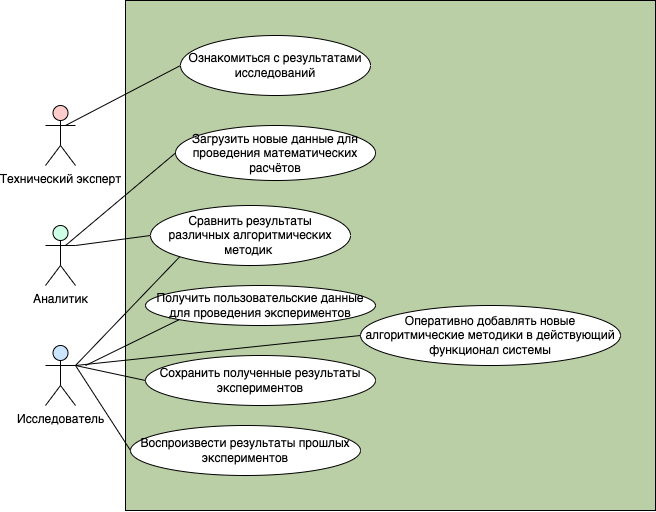
\includegraphics[width=0.6\textwidth, left]{analysis/pictures/usecases/usecase}
	\caption{Диаграмма вариантов использования}
	\label{pic:analysis__usecases-usecase}
\end{figure}
\vskip 5 mm



\section{Анализ предметной области}

\begin{frame}
\frametitle{Варианты использования}
\begin{figure}
    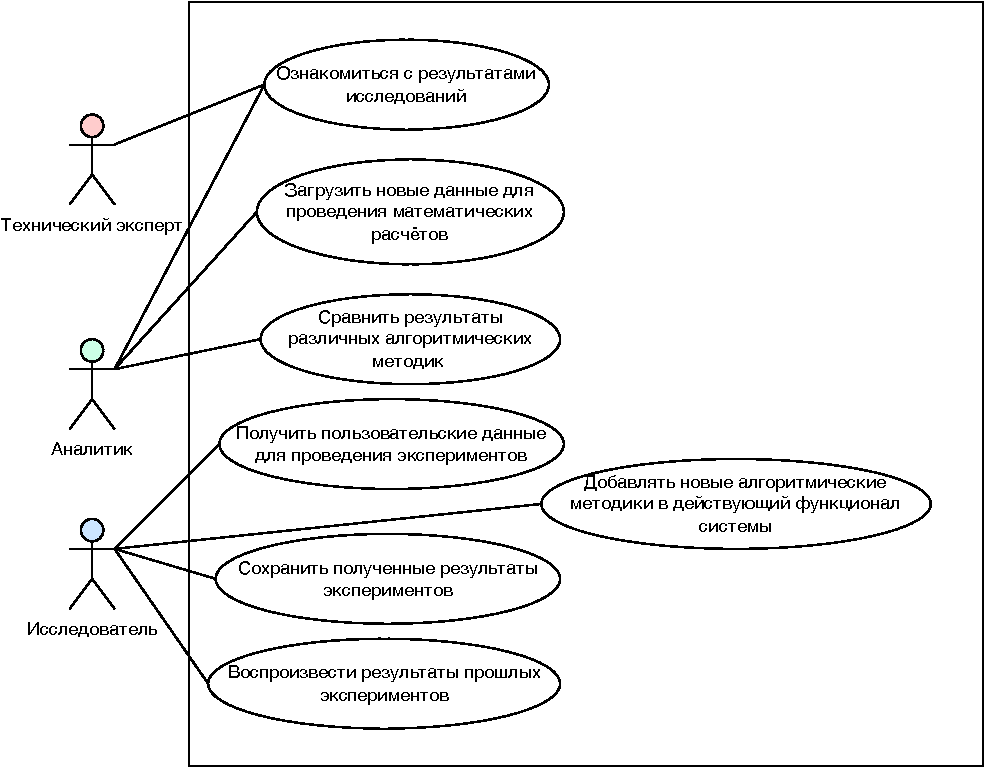
\includegraphics[scale=.48]{pictures/analysis/usecase}
    \caption{Диаграмма вариантов использования}
\end{figure}
\end{frame}

\begin{frame}
\frametitle{Бизнес-процессы}
\begin{figure}
    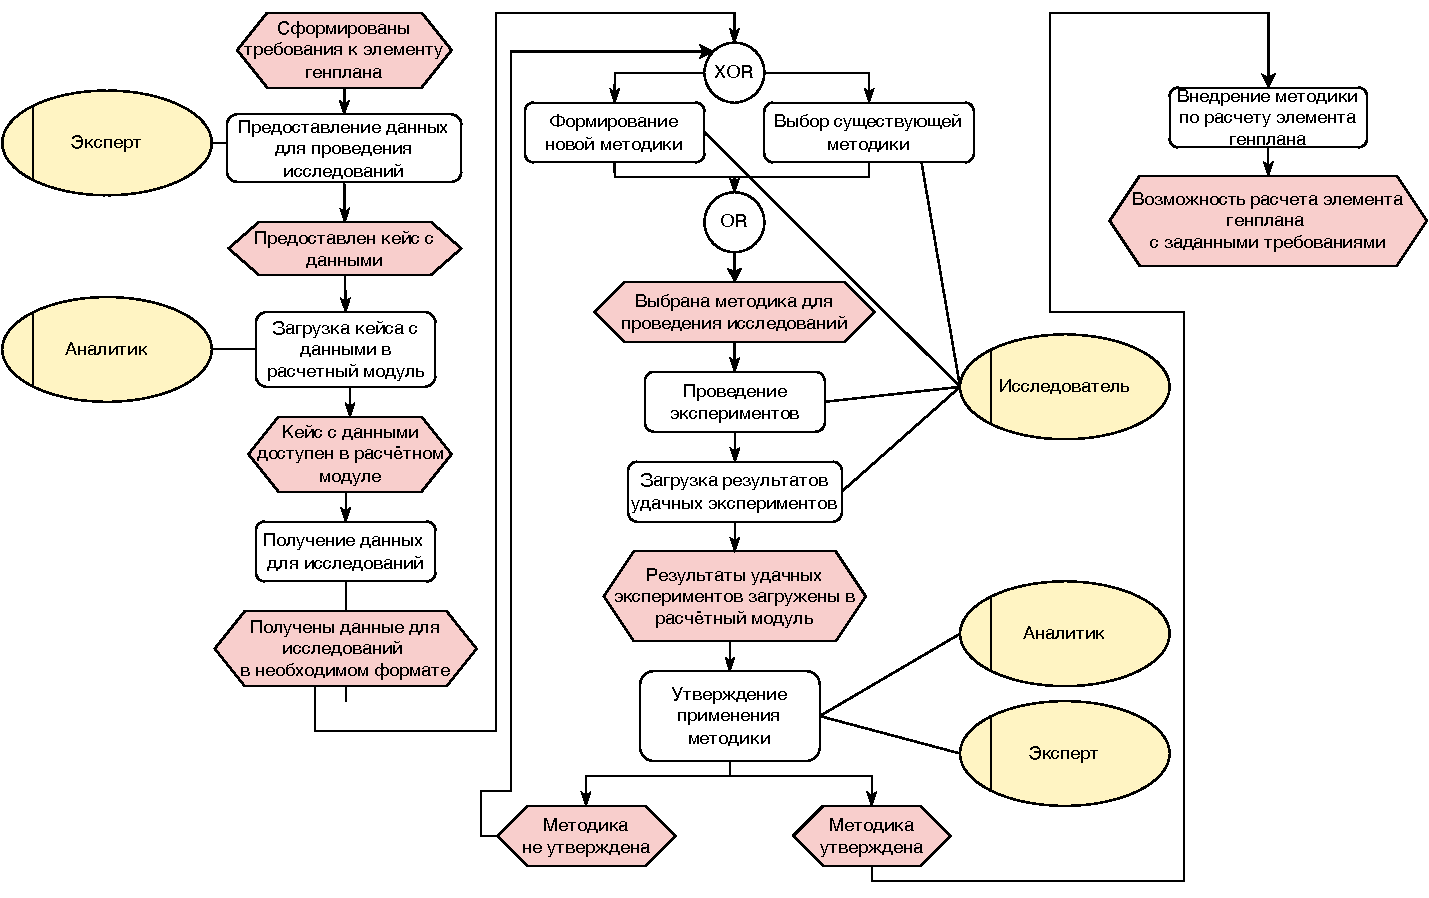
\includegraphics[scale=.48]{pictures/analysis/common_epc}
\end{figure}
\end{frame}

%\begin{frame}
%\frametitle{Бизнес-процессы}
%\begin{figure}
%    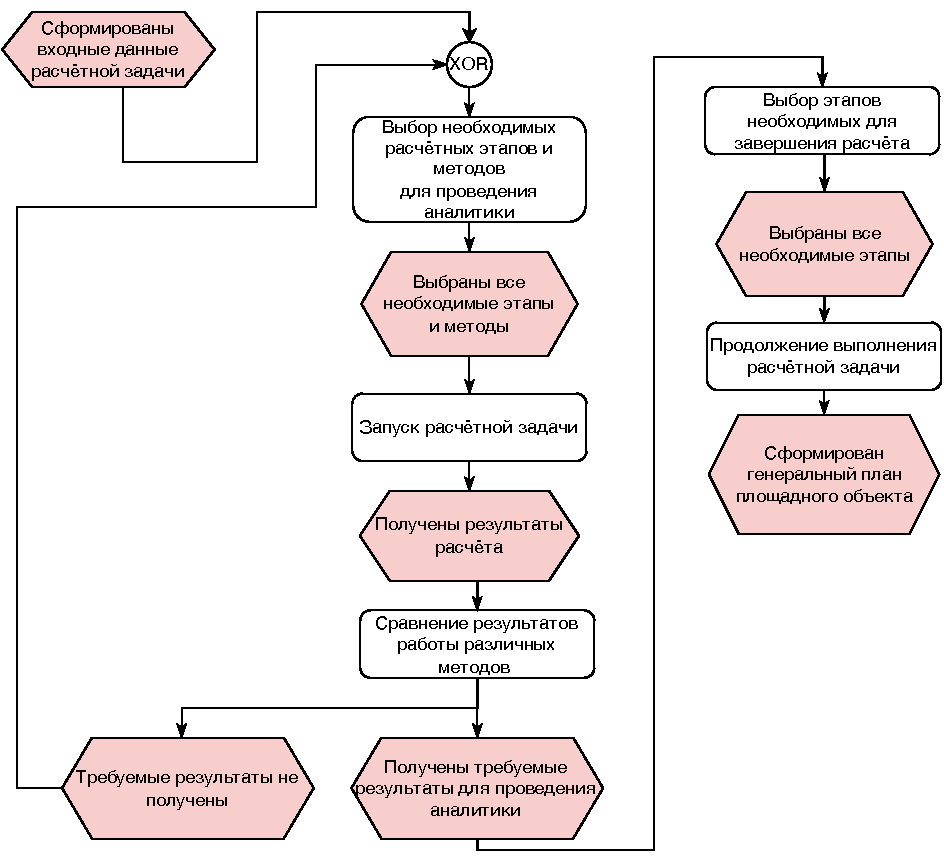
\includegraphics[scale=.49]{pictures/analysis/analytics_epc}
%\end{figure}
%\end{frame}


\begin{frame}
\frametitle{Предметная область задачи}
\begin{columns}[c]

\column{.45\textwidth}{
    Входные данные
    \begin{itemize}
        \item допустимая для строительства область на карте;
        \item стоимостная модель расчета стоимости инженерной подготовки;
        \item перечень сооружений;
        \item параметры коммуникаций между сооружениями проектируемого объекта;
        \item параметры цифровой модели рельефа;
    \end{itemize}
}

\column{.45\textwidth}{
    Выходные данные
    \begin{itemize}
        \item фигура площадного объекта;
        \item местоположения сооружений;
        \item схема технологических эстакад минимальной длины;
        \item схема внутриплощадочных проездов;
        \item стоимость инженерной подготовки;
        \item зоны распространения теплового потока;
        \item зоны распространения взрывной волны;
    \end{itemize}
}
\end{columns}
\end{frame}


\section{Формирование требований}

\begin{frame}
\frametitle{Функциональные требования}
\begin{enumerate}
    \item {
        Возможность расчёта генерального плана площадного объекта в автоматическом режиме.
    }
    \item {
        Расчёт генплана должен представлять последовательность этапов.
    }
    \item {
        Результат каждого этапа расчёта должен быть сохранён в долговременное хранилище.
    }
    \item {
        Возможность продолжить расчёт с последнего успешно завершенного этапа.
    }
    \item {
        Возможность сравнения одинаковых расчётных объектов, полученных путем применения различных методик.
    }
    \item {
        Возможность загрузки данных, полученных от технических экспертов, в расчётный модуль.
    }
    \item {
        Возможность загрузки результатов экспериментов, а также информации об особенностях
        проведения экспериментов в расчётный модуль.
    }
\end{enumerate}
\end{frame}


\begin{frame}
\frametitle{Нефункциональные требования}
\begin{enumerate}
    \item {
        Проведение исследований на вычислительном сервере с операционной системой Ubuntu 20.04 LTS.
    }
    \item {
        Осуществление вызова алгоритмически сложной части системы в отдельном процессе.
    }
    \item {
        Разработанные алгоритмы должны быть оформлены в отдельную библиотеку, имеющей версионирование.
    }
    \item {
        Обеспечение высокой скорости добавления алгоритмических методик в проект.
    }
    \item {
        Обеспечение высокого уровня гибкости системы.
    }
\end{enumerate}
\end{frame}

\section*{\large{Архитектура сервиса}}
\addcontentsline{toc}{section}{Архитектура сервиса}

На диаграмме размещения системы(см. рис\ \ref{pic:architecture__deployment-diagram}) расчетный сервис выделен голубым цветом.

\begin{figure}[H]
	\hspace*{-1 cm}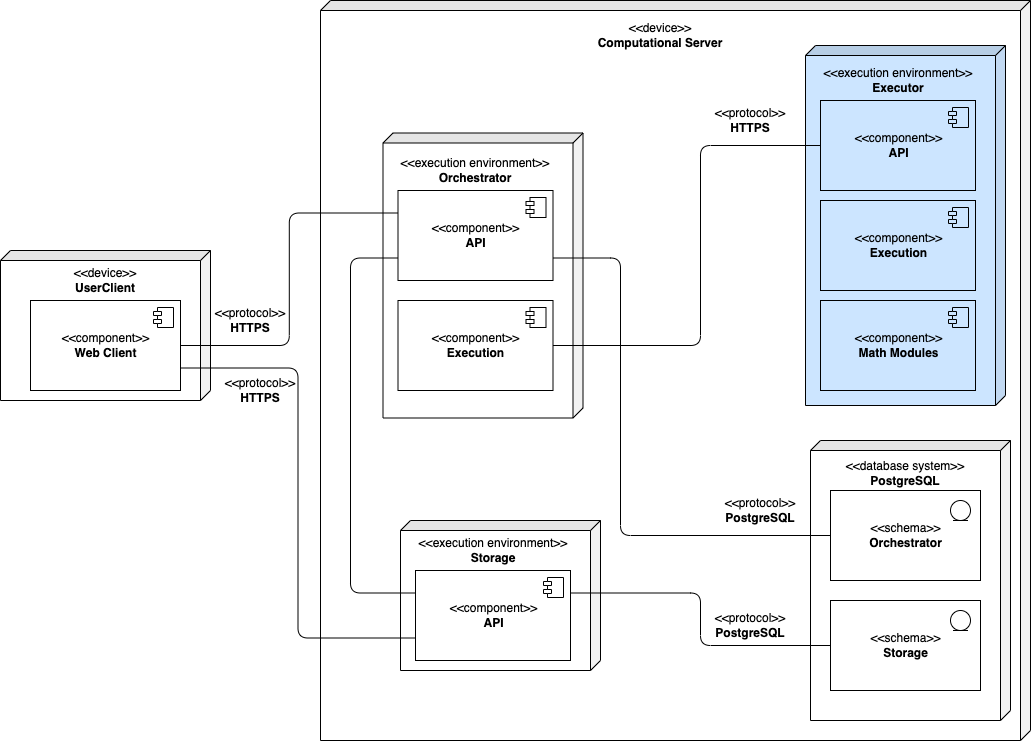
\includegraphics[width=\textwidth]{images/architecture/deployment_diagram}
	\caption{Диаграмма размещения}
	\label{pic:architecture__deployment-diagram}
\end{figure}
\vskip 5 mm

Расчетный сервис представлен тремя компонентами: API, расчётным модулем и математической библиотекой \textbf{nd\_plan}.
В качестве цели данной работы является проектирование и разработка API и расчетного модуля,
то поэтому только они и отражены на диаграммах ниже.

\begin{figure}[H]
	\hspace*{-2.5 cm}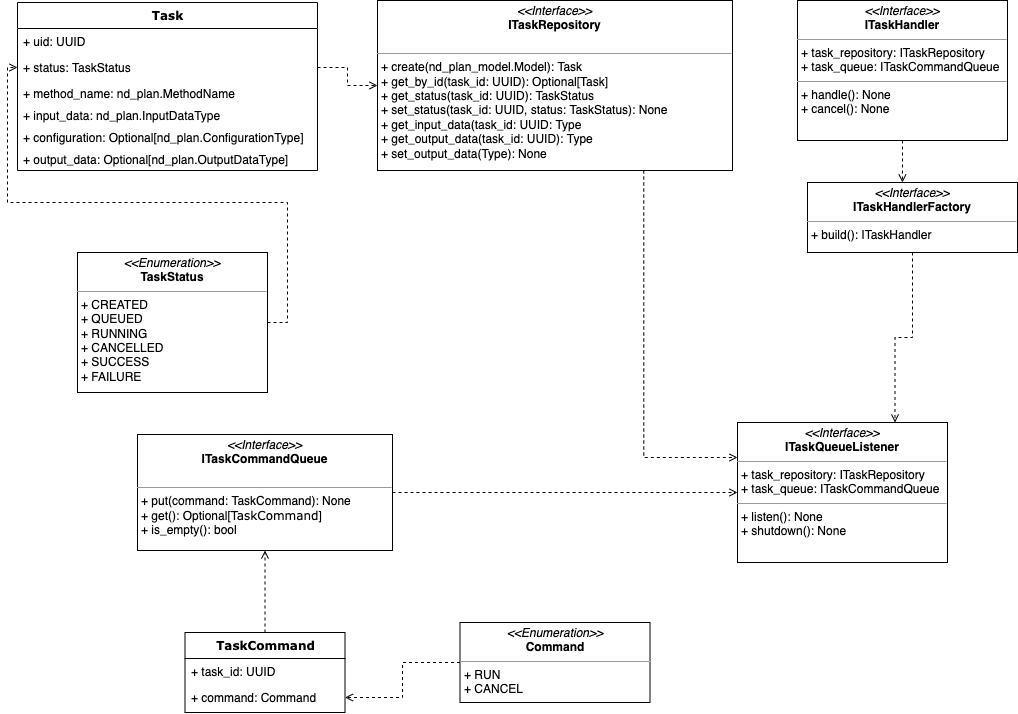
\includegraphics[width=1.2\textwidth]{images/architecture/execution_classes_diagram}
	\caption{Диаграмма классов расчетного модуля}
	\label{pic:architecture__execution-classes-diagram}
\end{figure}

\vskip 5 mm
Основное ядро бизнес-логики проекта представлено на диаграмме классов(см. рис\ \ref{pic:architecture__classes-diagram}).
Основные классы и интерфейсы:
\begin{enumerate}
	\item \textit{ITilesCacheStorage} -- сервис, отвечающий за кэширование векторных тайлов.
	\item \textit{ITilesRenderer} -- сервис, отвечающий за рендеринг векторных тайлов.
	\item \textit{ITilesDataProvider} -- сервис, отвечающий за получение данных из внешних источников для рендеринга.
	\item \textit{ITilesRepository} -- оркестратор, отвечает за получение отрендеренных тайлов.
	Если тайла нет в кэше, то он с помощью \textit{ITilesDataProvider} получает данные для рендеринга, потом
	с помощью \textit{ITilesRenderer} рендерит тайлы, а после сохраняет их в кэш \textit{ITilesCacheStorage}.
	\item \textbf{TileInfo} -- хранит в себе координаты запрашиваемого тайла, а также уникальный идентификатор генплана.
	\item \textbf{TileData} -- хранит в себе сырые данные, запрошенные по \textbf{TileInfo}.
	Из сырых данных генерируется \textbf{MapboxVectorTile}.
	\item \textbf{TileConfiguration} -- хранит в себе параметры слоев, которые требуется получить из источника данных.
	\item \textbf{MapboxVectorTile} -- хранит в себе данные, соответствующие спецификации \textit{Mapbox Vector Tile 2.1}.
\end{enumerate}


\begin{figure}[H]
	\hspace*{-2.5 cm}\includegraphics[width=1.2\textwidth]{images/architecture/}
	\caption{Диаграмма классов API}
	\label{pic:architecture__api-classes-diagram}
\end{figure}


\section*{\Large{РЕАЛИЗАЦИЯ}}
\addcontentsline{toc}{section}{РЕАЛИЗАЦИЯ}

При реализации описанной архитектуры была получена следующая структура
проекта(см. рисунок \ref{pic:implementation__packages}).

\begin{figure}[H]
	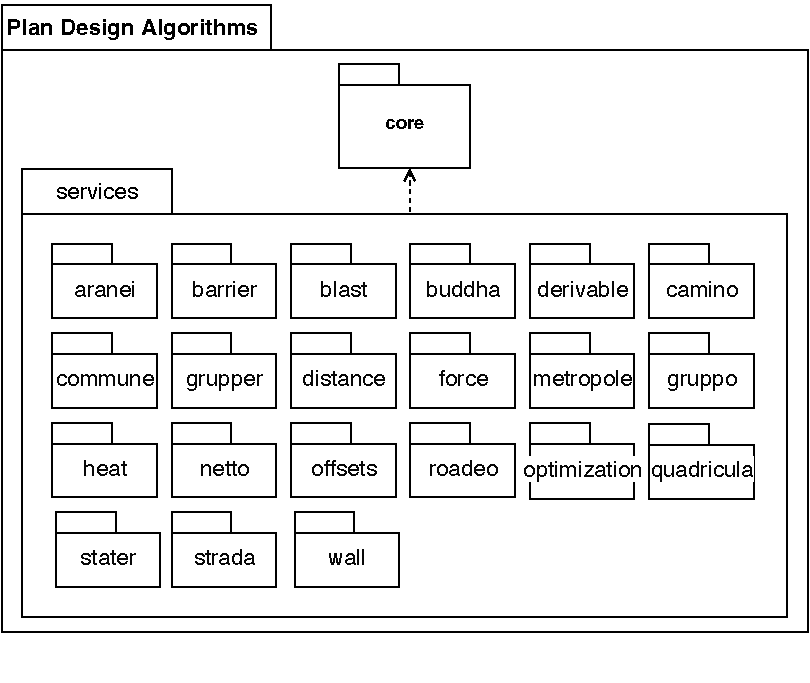
\includegraphics[width=0.6\textwidth]{pictures/packages}
	\caption{Диаграмма пакетов сервиса запуска расчётных задач}
	\label{pic:implementation__packages}
\end{figure}
\vskip 5 mm

Всего получилось 6 python-пакетов, в которых и скрыта основная логика работы.
\begin{enumerate}
    \item \textit{api} -- реализует API сервисы через HTTP. То есть endpoint-ы,
    модели запросов/ответов к серверу, а также взаимодействие с \textit{ITaskRepository} и \textit{ITaskDataManager}
    \item \textit{database} -- обеспечивает взаимодействие с базой данных.
    \item \textit{clients} -- пакеты, в котором находятся клиенты для взаимодействия с сервисами хранилища и сервиса 
    запуска математических методов.
    \item \textit{domain} -- пакет, в котором определены только интерфейсы взаимодействия между модулями программы.
    Непосредственная реализация обозначенных интерфейсов находится в других пакетах.
    \item \textit{execution} -- пакет, в котором находится код, отвечающий за запуск расчётных задач.
    \item \textit{repositories} -- пакет, который обеспечивает логику сохранения/получения сущностей проекта из БД.
\end{enumerate}

\subsection*{\Large{Примеры кода}}
\addcontentsline{toc}{subsection}{Примеры кода}

\begin{lstlisting}[language=Python, caption=main.py, captionpos=b]
from app import startup_app
import uvicorn

if __name__ == '__main__':
    app = startup_app()
    uvicorn.run(app, host="0.0.0.0", port=8080)
\end{lstlisting}

\vskip 10 mm
\begin{lstlisting}[caption=Dockerfile, captionpos=b]]
FROM python:3.8@sha256:4c4e6735f46e7727965d1523015874ab08f71377b3536b8789ee5742fc737059

WORKDIR /app

ENV LC_ALL C.UTF-8
ENV LANG C.UTF-8
ENV N_WORKERS 8

COPY requirements.txt .
RUN pip3 install --no-cache-dir -r requirements.txt

RUN pip3 check

COPY main.py .

COPY /app ./app

ENTRYPOINT /bin/bash -c "gunicorn run_app:app --workers=${N_WORKERS} --bind 0.0.0.0:8080 --worker-class aiohttp.GunicornWebWorker --timeout 0"
\end{lstlisting}

\vskip 10 mm
\begin{lstlisting}[language=Python, caption=domain/model.py, captionpos=b]
class Status(Enum):
    CREATED = "CREATED"
    QUEUED = "QUEUED"
    RUNNING = "RUNNING"
    CANCELLED = "CANCELLED"
    SUCCESS = "SUCCESS"
    FAILURE = "FAILURE"


@dataclass
class Feature:
    id: UUID = UUID(int=0)
    feature_type_id: UUID = UUID(int=0)


@dataclass
class Method:
    id: UUID = UUID(int=0)
    method_type_id: UUID = UUID(int=0)
    status: Status = Status.CREATED


@dataclass
class Calculation:
    id: UUID = UUID(int=0)
    calculation_type_id: UUID = UUID(int=0)
    status: Status = Status.CREATED


@dataclass
class Stage:
    id: UUID = UUID(int=0)
    stage_type_id: UUID = UUID(int=0)
    status: Status = Status.CREATED


@dataclass
class Task:
    id: UUID = UUID(int=0)
    name: str = ""
    task_type_id: UUID = UUID(int=0)
    status: Status = Status.CREATED
\end{lstlisting}
\vskip 10 mm


\section{Результаты}

\begin{frame}
\frametitle{Интерфейс системы}
\begin{figure}
    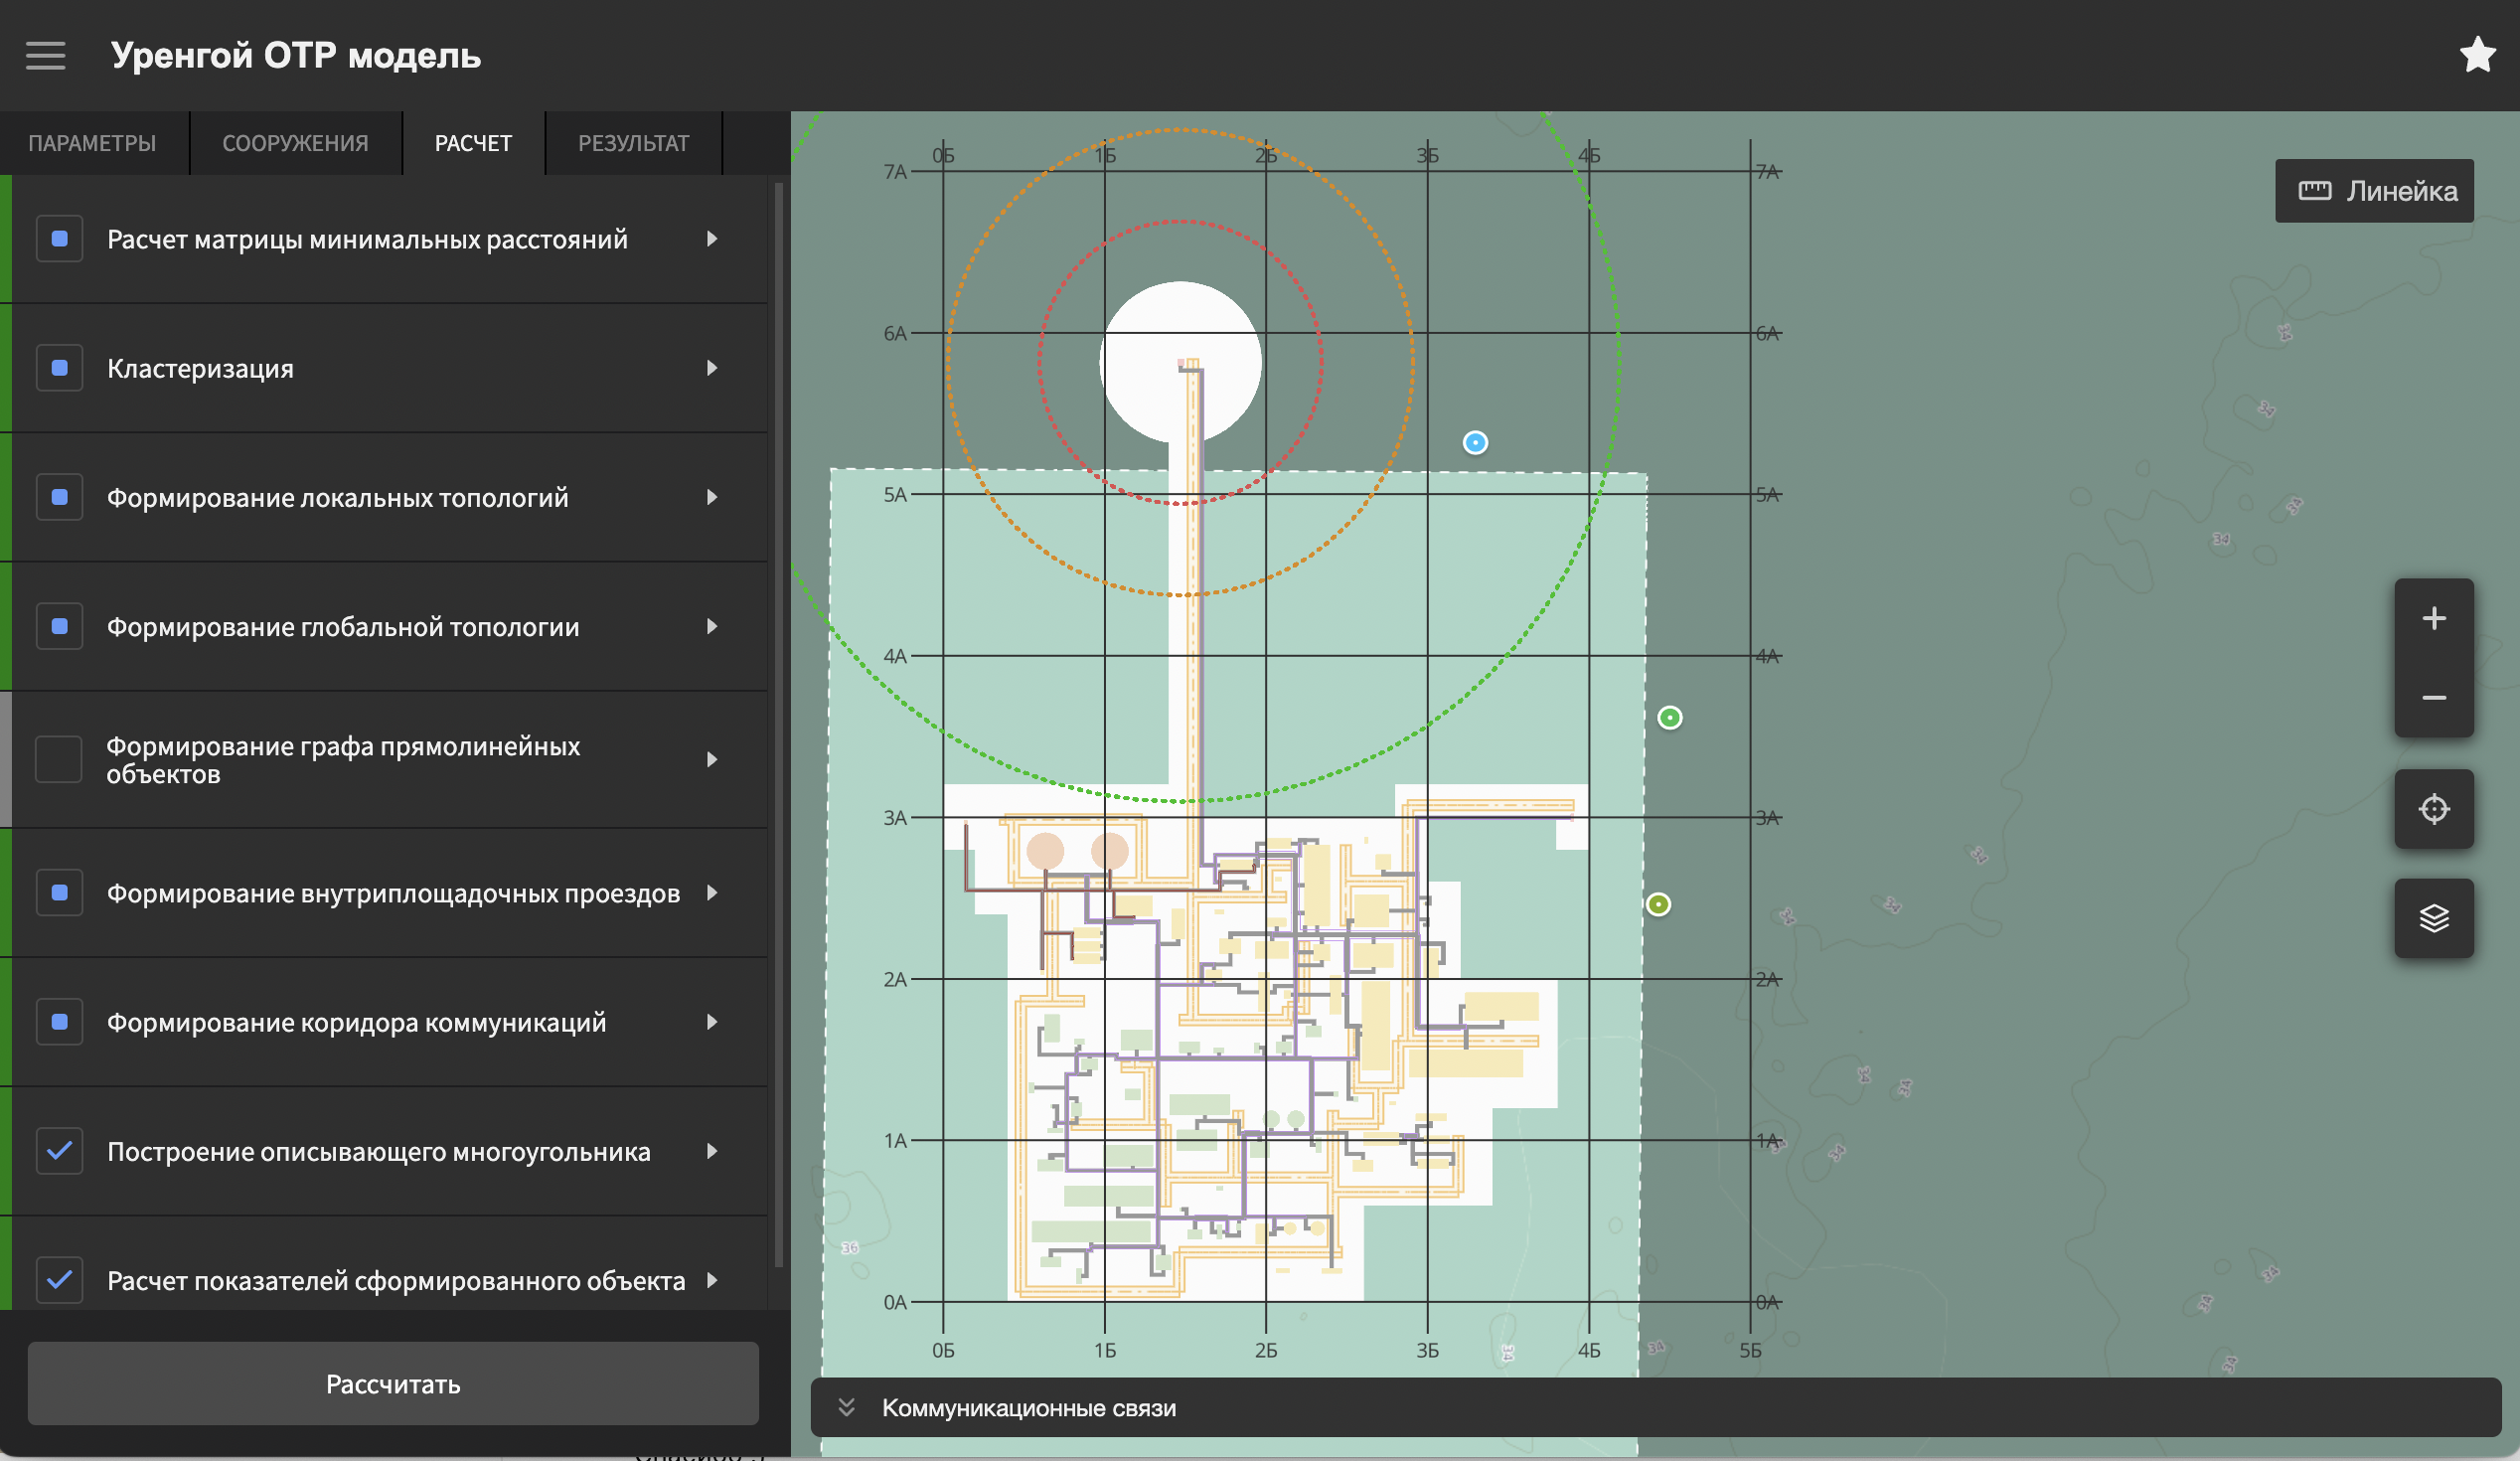
\includegraphics[scale=0.1391]{pictures/results/plan-system}
\end{figure}
\end{frame}


\begin{frame}
\frametitle{Результаты}
\begin{itemize}
    \item собраны и проанализированы требования пользователей;
    \item сформированы функциональные и нефункциональные требования к программному компоненту;
    \item cпроектирована системная и программная архитектура расчётного модуля;
    \item {
           реализован расчётный модуль, состоящий из пяти программных компонент:
            \begin{enumerate}
                \item математическая библиотека,
                \item расчётная модель данных,
                \item сервис запуска расчётных задач,
                \item сервис хранения расчётных данных,
                \item сервис запуска математических методов.
            \end{enumerate}
    }
\end{itemize}
\end{frame}



\begin{frame}[plain]
    \itmopolygons{
        \vfill
        \Huge{Спасибо за внимание!}
        \vfill
        
\includegraphics[scale=.5]{itmo/slogan}
    }
\end{frame}

\appendix
\section{Приложения}

\begin{frame}
\frametitle{Тестирование}
\begin{figure}
Общее покрытие тестами составляет около 50\%.
\begin{itemize}
    \item Математическая библиотека 53\%
    \item Сервис запуска расчётных задач 46\%
    \item Сервис запуска математических методов 54\%
    \item Сервис хранилища расчётных данных 49\%
\end{itemize}
\end{figure}
\end{frame}


\begin{frame}
\frametitle{Диаграмма развёртывания}
\begin{figure}
    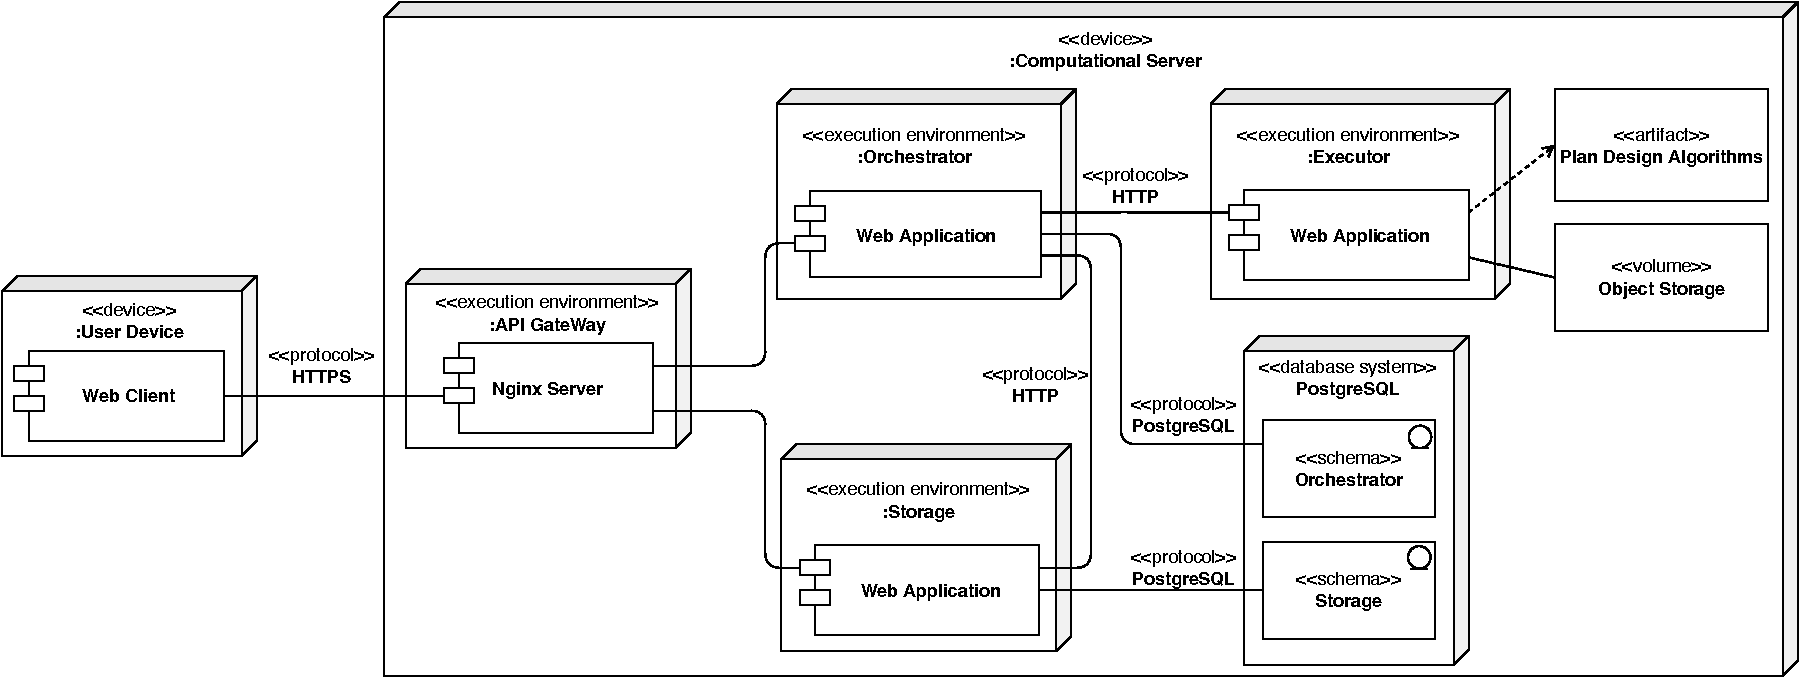
\includegraphics[scale=.49]{pictures/architecture/deployment}
\end{figure}
\end{frame}

\begin{frame}
\frametitle{Диаграмма классов расчётной модели}
\begin{figure}
    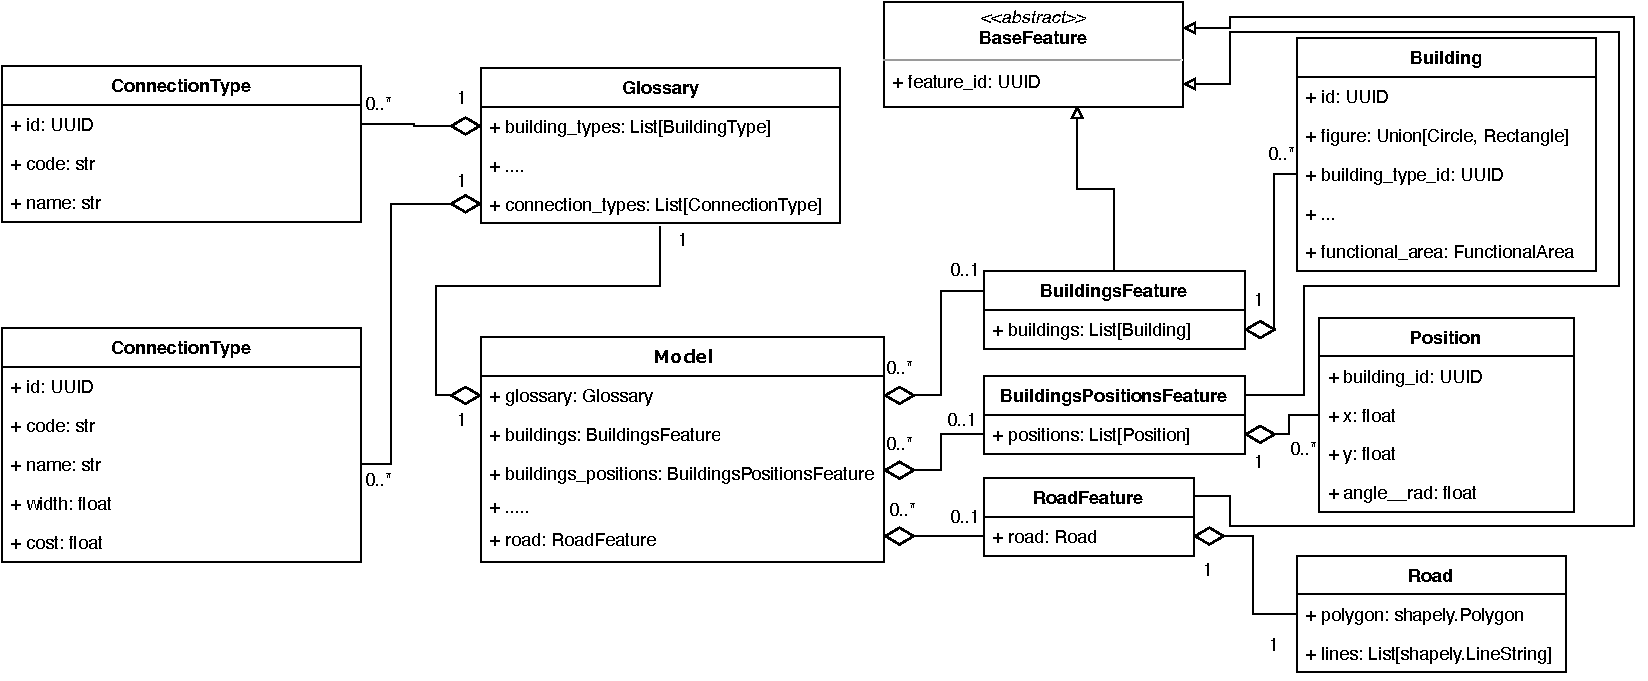
\includegraphics[scale=.54]{pictures/implementation/appendix_classes}
\end{figure}
\end{frame}


\begin{frame}
\frametitle{Диаграмма пакетов математической библиотеки}
\begin{figure}
    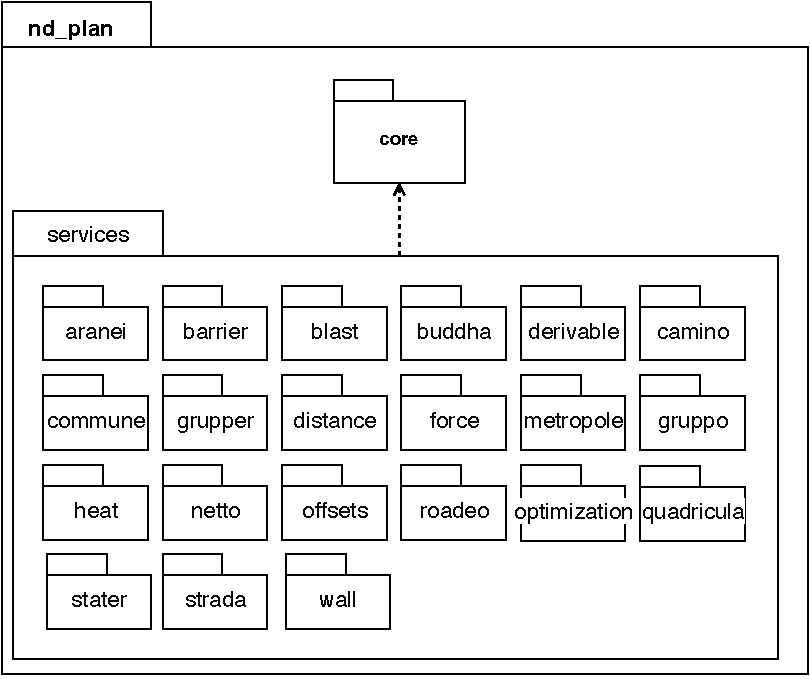
\includegraphics[scale=.49]{pictures/implementation/math_packages}
\end{figure}
\end{frame}

\begin{frame}
\frametitle{Сервис запуска математических методов}
\begin{figure}
    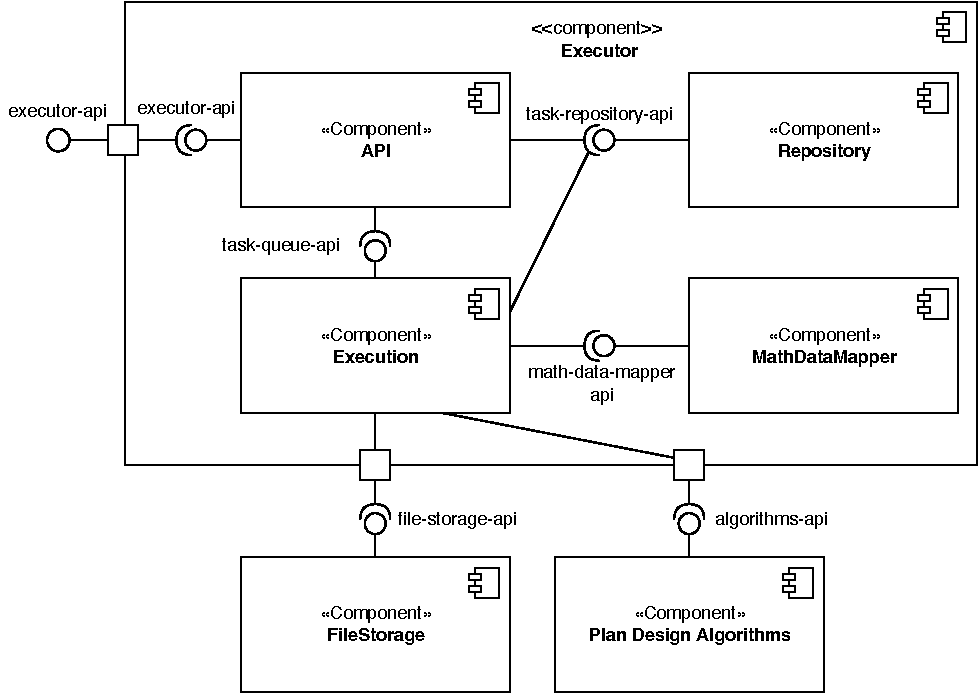
\includegraphics[scale=.6]{pictures/architecture/executor_component_common}
\end{figure}
\end{frame}

\begin{frame}
\frametitle{Компонент запуска математических методов}
\begin{figure}
    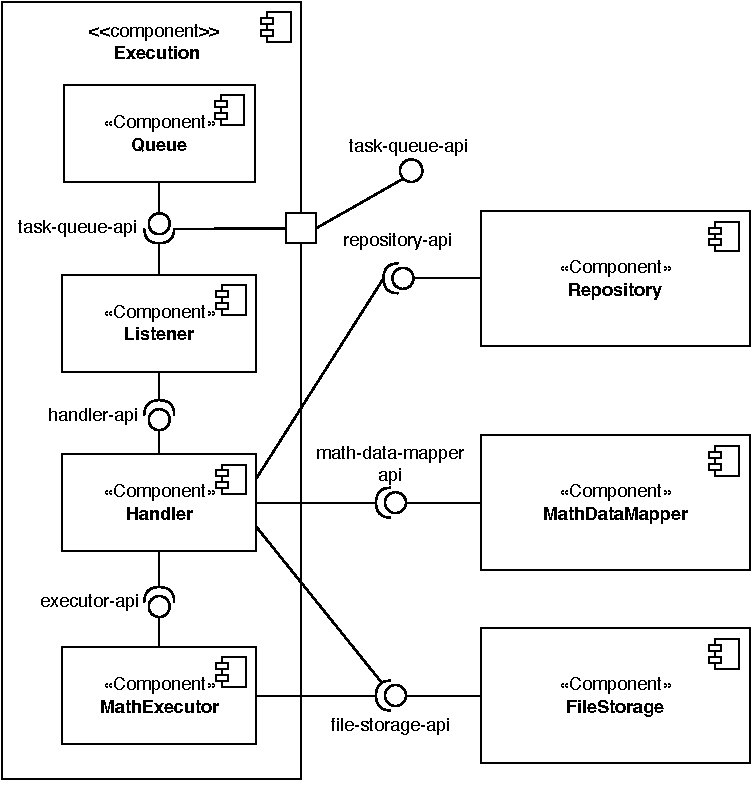
\includegraphics[scale=.5]{pictures/architecture/executor_component_detailed}
\end{figure}
\end{frame}

\begin{frame}
\frametitle{Хранилище расчётных данных}
\begin{figure}
    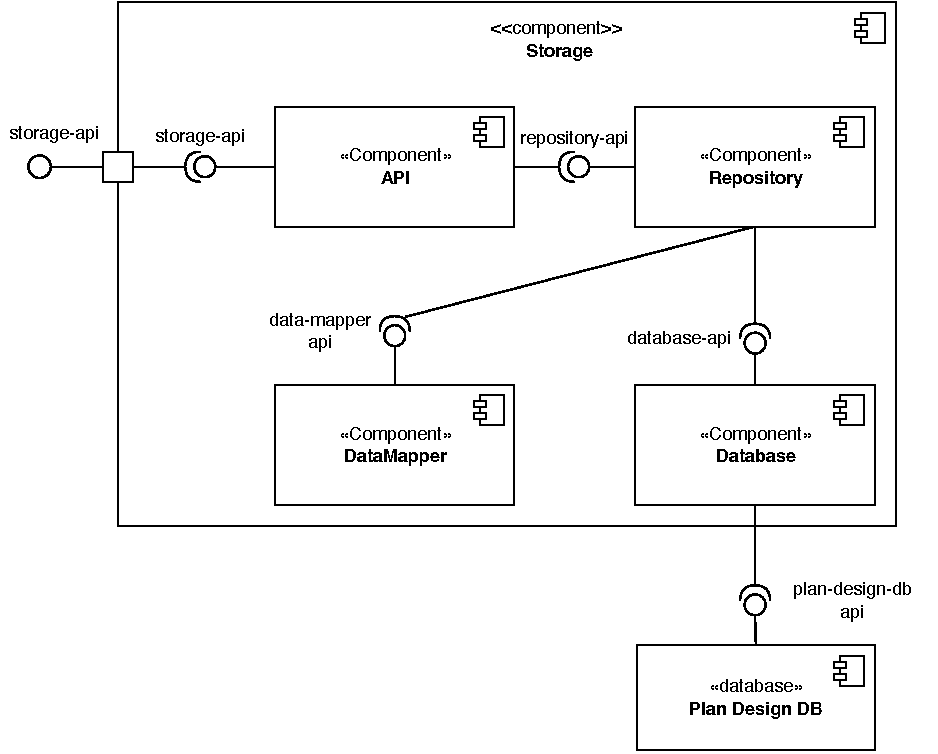
\includegraphics[scale=.55]{pictures/architecture/storage_component_common}
\end{figure}
\end{frame}


\begin{frame}
\frametitle{Компонент запуска расчётных задач}
\begin{figure}
    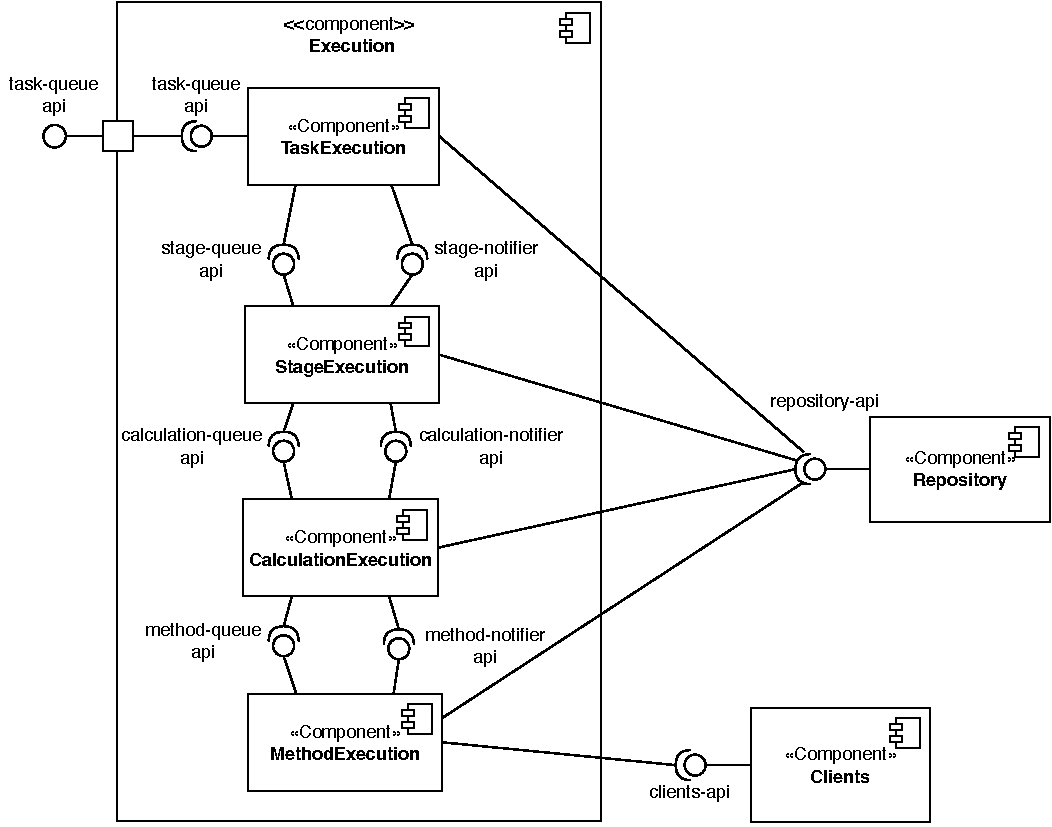
\includegraphics[scale=.5]{pictures/architecture/orchestrator_component_detailed}
\end{figure}
\end{frame}


\begin{frame}
\frametitle{Технологический стек}
\begin{itemize}
    \item Операционная система \textit{Ubuntu 20.04 LTS}
    \item Язык программирования \textit{Python 3.8.12}
    \item База данных \textit{PostgreSQL 12} с расширением \textit{PostGIS 3.1}
    \item Веб-сервер \textit{nginx}
    \item Автоматическое развертывание \textit{Gitlab-CI}
    \item Контейнеризация \textit{Docker} и \textit{docker-compose}
    \item Документация \textit{OpenAPI} и \textit{LaTex}
    \item Система сборки логов \textit{ELK}
    \item Протоколы взаимодействия \textit{REST API over HTTP}
    \item Формат данных \textit{JSON}
\end{itemize}
\end{frame}


\begin{frame}
\frametitle{Варианты использования}
\begin{figure}
    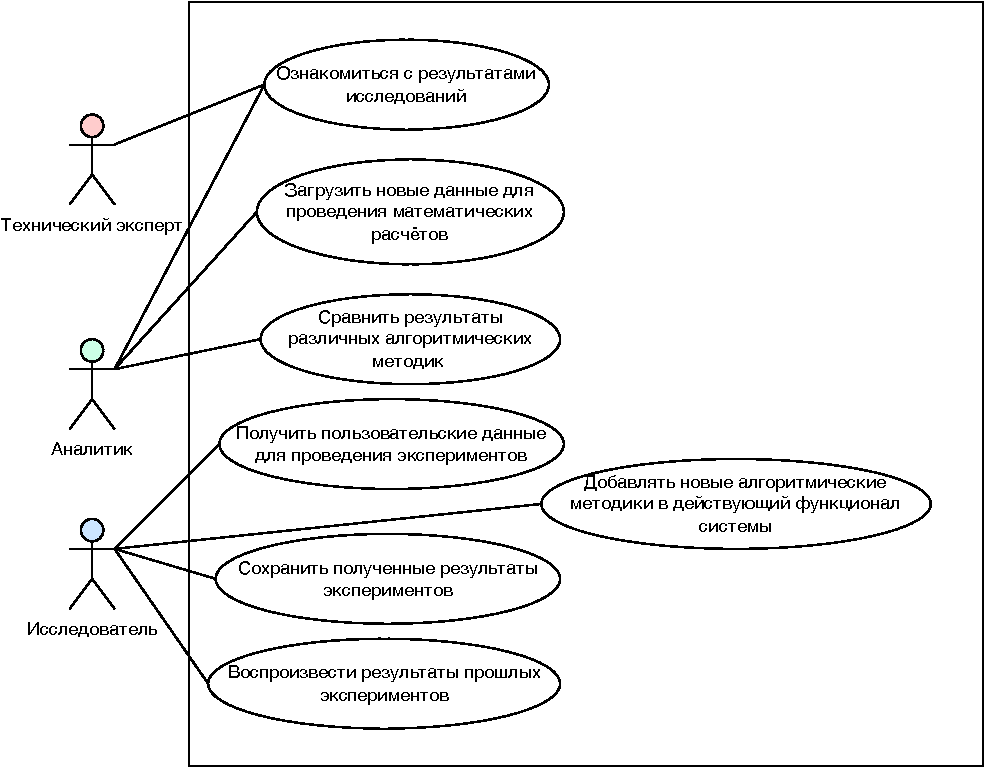
\includegraphics[scale=.48]{pictures/analysis/usecase}
    \caption{Диаграмма вариантов использования}
\end{figure}
\end{frame}


\begin{frame}
\frametitle{Предметная область задачи}
\begin{columns}[c]

\column{.45\textwidth}{
    Входные данные
    \begin{itemize}
        \item допустимая для строительства область на карте;
        \item стоимостная модель расчета стоимости инженерной подготовки;
        \item перечень сооружений;
        \item параметры коммуникаций между сооружениями проектируемого объекта;
        \item параметры цифровой модели рельефа;
    \end{itemize}
}

\column{.45\textwidth}{
    Выходные данные
    \begin{itemize}
        \item фигура площадного объекта;
        \item местоположения сооружений;
        \item схема технологических эстакад минимальной длины;
        \item схема внутриплощадочных проездов;
        \item стоимость инженерной подготовки;
        \item зоны распространения теплового потока;
        \item зоны распространения взрывной волны;
    \end{itemize}
}
\end{columns}
\end{frame}

%\input{samples.tex}

\end{document}
